Database testing is performed in a dynamic white-box manner. The tests are white-box as it is not the MySQL server we are testing, but that the database design
correspond to functionally that are expecting.A total of 16 test cases have been designed, \autoref{fig:dbtest01-12} show the test design for test cases \#00 to \#11.
The identifier TD0001 points \autoref{fig:dbtd0001}, which explains each step to be performed for the test cases in \autoref{fig:dbtest01-12}.


\begin{figure}[H]
 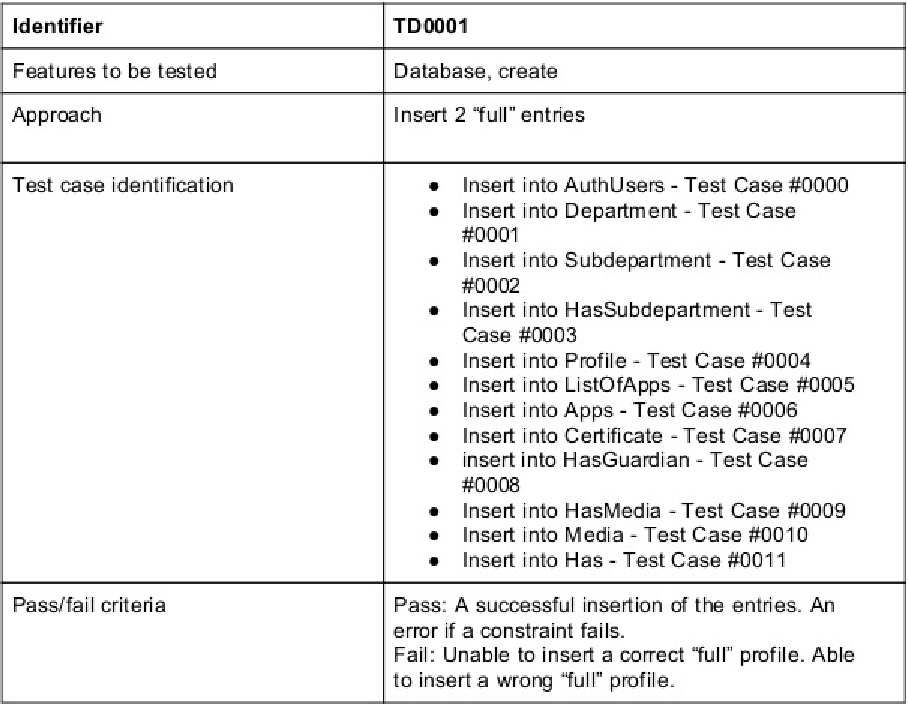
\includegraphics[scale=1.00]{images/dbtesttd0001}
 \caption{Testcase design of tests 01 to 12.}
  \label{fig:dbtest01-12}
\end{figure}

\begin{figure}[H]
 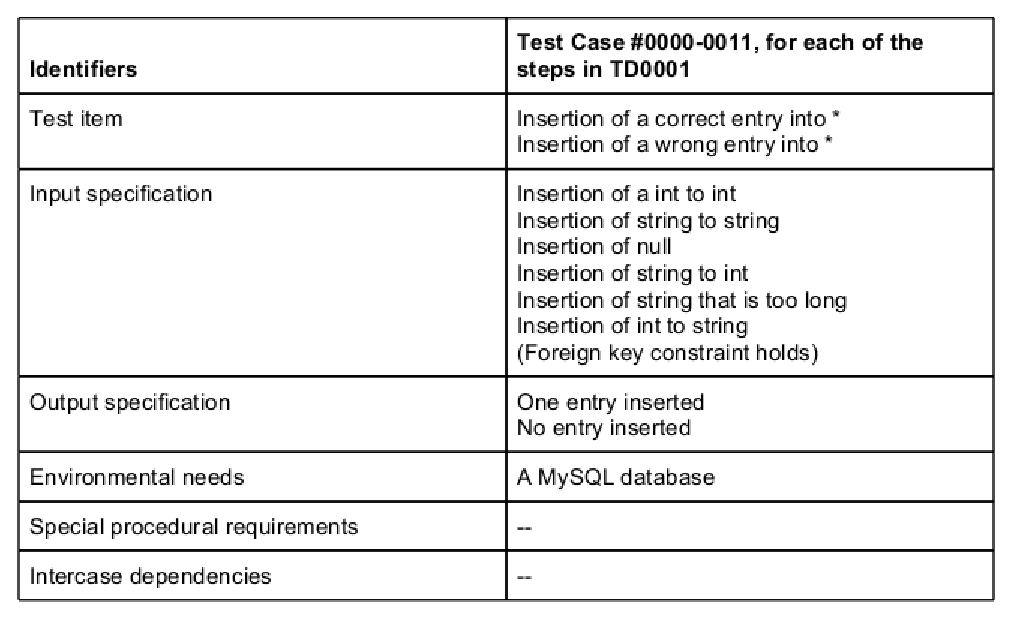
\includegraphics[scale=1.00]{images/dbtestcase01-12}
  \caption{Testcases 01 to 12}
  \label{fig:dbtd0001}
\end{figure}

All the database tests are done manually through a terminal and thus require human interpretation \autoref{hej}


\begin{Code}
\begin{lstlisting}[label=hej,caption=ninja]
--------------
INSERT INTO AuthUsers
values('tolongstring',null,1,
       'username00username00username00username00username00',
       'hansen')
--------------

ERROR 1406 (22001): Data too long for column 'username' at row 1
ERROR 1064 (42000): You have an error in your SQL syntax;
                    check the manual that corresponds
                    to your MySQL server version for the right 
                    syntax to use near 'INT(2))' at line 1
\end{lstlisting}
\end{Code}







